% LaTeX-Vorlage zur Erstellung von Abschlussarbeiten an der FH Aachen
% Author: Sven Hinz
% Aenderung für FB 5: Ingo Elsen
\documentclass[11pt, a4paper, headinclude, footinclude=true, oneside]{scrreprt}
% Paket für Umlaute:
\usepackage[utf8]{inputenc}       % Cross Platform
%\usepackage[ansinew]{inputenc}   % Windows
%\usepackage[latin1]{inputenc}    % Linux
%\usepackage[applemac]{inputenc}  % Mac

\usepackage[USenglish]{babel}       % Sprache: US English
\usepackage[utf8]{inputenc} % For degree symbol in tex source
\usepackage{amsmath}
\usepackage{amsfonts}
\usepackage{amssymb}
\usepackage{makeidx}
\usepackage{graphicx}
\usepackage{epstopdf}
%\usepackage{kpfonts}
%\usepackage{textcomp}
\usepackage[left=3cm,right=3cm,top=2.5cm,bottom=2.5cm]{geometry}
%\usepackage[plainheadsepline,headsepline]{scrpage2}
\usepackage{color}
\usepackage{xcolor}
\usepackage{setspace}
%\usepackage[numbers,square]{natbib} % only required for unsrtd bib style
\usepackage{longtable}
\usepackage{tabularx}
\usepackage{listings}
\usepackage{rotating}
\usepackage{pdfpages}
\usepackage{caption}
\usepackage{subcaption}
\parindent 0pt
\usepackage{booktabs}
\usepackage[export]{adjustbox}
\usepackage{scrlayer-scrpage}
\usepackage{float} % for right positioning of pictures


% Schriftart
\usepackage{courier}
\usepackage{helvet}
\usepackage{times}
%\renewcommand{\familydefault}{\sfdefault}
%\renewcommand{\familydefault}{\rmdefault}
%\setkomafont{chapter}{\sffamily \large}
%\setkomafont{section}{\sffamily \normalsize}
%\setkomafont{subsection}{\sffamily \normalsize}
%\setkomafont{subsubsection}{\sffamily \normalsize}
%\addtokomafont{caption}{\sffamily \small}


% Abstand zwischen Kopfzeile und Kapitelüberschrift
%\renewcommand*{\chapterheadstartvskip}{\vspace*{-0.75\baselineskip}}

% Einstellungen der Kopf- und Fußzeile
\pagestyle{scrheadings}
%\ihead[\sffamily \bfseries \upshape \headmark]{\sffamily \bfseries \upshape \headmark}
\ohead[\sffamily \bfseries \upshape \headmark]{\sffamily \bfseries \upshape \headmark}
\chead[]{}
\ohead[]{}
\ifoot[]{}
\cfoot[]{}
\ofoot[\sffamily \pagemark]{\sffamily \pagemark}
\automark[]{chapter}
\renewcommand*{\chapterheadendvskip}{\vspace*{1\baselineskip}}

% Formeln
%\usepackage{fleqn} % linksbündig
%\setlength{\mathindent}{1.5cm} % Einrücktiefe

% Tabellen
\usepackage{multirow} % mehrzeiliger Text in einer Spalte
\renewcommand{\arraystretch}{2} % Zeilenabstand vergrößern
\setlength{\doublerulesep}{0.1mm} % Abstand der Doppellinien verkleinern
\usepackage{tabu}
\newcolumntype{C}{>{\centering\arraybackslash$}p{3cm}<{$}}

% Quellcode / Kommandozeileneingabe
\lstdefinestyle{BashInputStyle}{
language=bash,
  basicstyle=\small\ttfamily,
  numbers=left,
  numberstyle=\tiny,
  numbersep=3pt,
  frame=tb,
  columns=fullflexible,
  backgroundcolor=\color{yellow!20},
  linewidth=0.9\linewidth,
  xleftmargin=0.1\linewidth
}

% Define Flux language for listings
\lstdefinelanguage{Flux}{
	morekeywords={
		import, from, range, filter, map, reduce, group, aggregateWindow,
		mean, sum, count, window, every, start, stop, pivot, join, drop,
		keep, yield, to, option, package, pipe, as, pivot, union
	},
	sensitive=true,
	morecomment=[l]{//},
	morecomment=[s]{/*}{*/},
	morestring=[b]",
	morestring=[b]',
	alsoletter={.},
}

% Flux listing style (use in preamble)
\lstdefinestyle{FluxStyle}{
	language=Flux,
	basicstyle=\small\ttfamily,
	keywordstyle=\color{blue}\bfseries,
	commentstyle=\color{gray}\itshape,
	stringstyle=\color{teal},
	numbers=left,
	numberstyle=\tiny,
	numbersep=6pt,
	frame=tb,
	columns=fullflexible,
	backgroundcolor=\color{yellow!20},
	linewidth=\textwidth,      % use full text width
	xleftmargin=0pt,          % no extra left margin
	xrightmargin=0pt,         % no extra right margin
	framexleftmargin=6pt,     % small padding between frame and text
	framexrightmargin=6pt,
	breaklines=true,
	breakatwhitespace=true,
	showstringspaces=false
}

% Inhalt
\renewcaptionname{USenglish}{\contentsname}{Contents} % Umbenennung in Inhalt

% Quellenverzeichnis
\renewcaptionname{USenglish}{\bibname}{Bibliography} % Umbenennung in Quellenverzeichnis

%\usepackage[
%  tocindentmanual,
%  tocflat,
%  tocbreaksstrict,
%  toctextentriesleft,
%]{tocstyle}

% Abkürzungsverzeichnis
%\usepackage[intoc]{nomencl}
%\let\abbrev\nomenclature
%\renewcommand{\nomname}{Abkürzungsverzeichnis}
%\setlength{\nomlabelwidth}{.25\hsize}
%\renewcommand{\nomlabel}[1]{#1 \dotfill}
%\setlength{\nomitemsep}{-\parsep}
%\makenomenclature

\usepackage[]{acronym}


\author{Nicolas Harrje} % --> Eigenen Namen einfügen


\begin{document}
\setstretch{1.1}
\addtocontents{toc}{\linespread{1}}

% Einbinden der Textinhalte mit '\include{...}'
% Die Dateien mit den Textinhalten befinden sich im Ordner 'doc'

\begin{titlepage}
	%ab hier kleinere Raender, mehr bedruckbare Flaeche.
	%\fontfamily{\sffamily}\selectfont
	\thispagestyle{empty}
	\newgeometry{a4paper, portrait, left=0cm, right=0cm, top=0.6cm, bottom=0cm, includefoot}

	% FH Logo
	\begin{flushright}
		
\includegraphics[width=1.7cm]{./pic/FHAC.jpg}
	\end{flushright}

	\vspace{-2.5cm}

	% Kopfzeile mit Fachbereich ...
	\centering \sffamily \bfseries \Large FH~Aachen \\
	\vspace{0.5cm}
	\normalsize Faculty\\
	Electrical engineering and information technology

	\vspace{1cm}

	%\centering \bfseries Bachelorarbeit
	\centering \bfseries Bachelor Thesis

	\vspace{0.8cm}

	%Titel der Arbeit
	\centering \begin{minipage}[t]{17cm}
		\centering \bfseries \large Design and Implementation of  a Performance Measurement System\\ for an Industrial Sewing Machine
		\medskip
	\end{minipage}

	\vspace{1.5cm}

	%Name und Matrikelnummer
	%\vspace*{1cm}
	%\hspace*{6.8cm}
	\begin{minipage}[t]{9cm}
		\centering Nicolas Harrje \\ Matr.-Nr.: 3518047
	\end{minipage}

	\vspace{2.1cm}

	%Professor und Betreuer
	%\vspace*{4.7cm}
	%\hspace*{6.8cm}
	\centering \begin{minipage}[t]{9cm}
		\centering \begin{tabular}{ll}
			Referent: & Prof. Dr-Ing. ...\\
			Korreferent: & Prof. Dr.-Ing. ...\\
			%Externer Betreuer: & Dipl.-Wirt.-Ing\\
		\end{tabular}
	\end{minipage}

	\vspace{7cm}

	% Firmenlogo
	%\begin{flushleft}
	%\centering \hspace{-8cm}
	%\begin{minipage}[t]{5cm}
			%\includegraphics[width=5cm]{./pic/firmenlogo.jpg}
	%\end{minipage}
	%\end{flushleft}


	%Erstellungsdatum
	%\vspace{-4cm}
	%\begin{flushright}
	\centering %\hspace{8cm}
	\begin{minipage}[b]{5cm}
			\centering
			\today\\ %Datum\\
			%\vspace{1cm}
			%In Zusammenarbeit mit\\
			%Firma, Ort\\
			%\vspace{1cm}
			%vertraulich bis xx.xx.xx
	\end{minipage}
	%\end{flushright}

	%\today
	\restoregeometry
\end{titlepage}


\clearpage
\chapter*{Erklärung}\label{erklaerung}
\markboth{Erklärung}{Erklärung}
Ich versichere hiermit, dass ich die vorliegende Arbeit selbstständig verfasst und keine anderen als die im Literaturverzeichnis angegebenen Quellen benutzt habe.

\bigskip

Stellen, die wörtlich oder sinngemäß aus veröffentlichten oder noch nicht veröffentlichten Quellen entnommen sind, sind als solche kenntlich gemacht.

\bigskip

Die Zeichnungen oder Abbildungen in dieser Arbeit sind von mir selbst erstellt worden oder mit einem entsprechenden Quellennachweis versehen.

\bigskip

Diese Arbeit ist in gleicher oder ähnlicher Form noch bei keiner anderen Prüfungsbehörde eingereicht worden.

\vspace{1cm}
Aachen, \today %Monat Jahr

\vspace{7cm}
\section*{Geheimhaltung - Sperrvermerk}\label{geheimhaltung}

Die vorliegende Arbeit unterliegt bis [Datum] der Geheimhaltung. Sie darf vorher weder vollständig noch auszugsweise ohne schriftliche Zustimmung des Autors, des betreuenden Referenten bzw. der Firma [Firmenname und -sitz] vervielfältigt, veröffentlicht oder Dritten zugänglich gemacht werden.

%\clearpage
\chapter*{Danksagung}\label{danksagung}
\markboth{Danksagung}{Danksagung}
Danke.

% Inhaltsverzeichnis
\clearpage
\makeatletter
\renewcommand*{\@dotsep}{1} % Punktabstand einstellen
\makeatother
\tableofcontents

% Das erste Kapitel soll auf einer ungeraden Seite beginnen.
\cleardoublepage
\setstretch{1.1}

% Nicht benötigte Kapitel können auskommentiert werden
% Für zusätzliche Kapitel müssen weitere Dateien im Ordner 'doc' angelegt werden

\clearpage
\chapter{\textbf{Introduction}}\label{introduction}
Industrial sewing machines are of crucial importance in the textile industry, where they are typically utilized in the final stage of production to assemble the end product. This stage necessitates the highest level of human involvement, thereby becoming a pivotal element in determining both production efficiency and product quality. Therefore, the implementation of performance measurement techniques is particularly appropriate in this context. In the field of performance measurement, the seminal work by Neely \cite{neelyPerformanceMeasurementSystem1995} is widely cited. They defined performance measurement as "[...] the process of quantifying the efficiency and effectiveness of action." . This is frequently achieved through the implementation of Key Performance Indicators (KPIs), as they are formally standardized in the ISO 22400 framework, which governs operations management and production.
\\\\
In recent years, the popularity of automatic systems for performance measurement on sewing machines has increased. Nonetheless, these systems continue to encounter certain challenges that have frequently been overlooked. Firstly, it must be acknowledged that a considerable number of systems are dependent on cloud technology. This reliance engenders certain issues, including elevated latency and the perpetual financial obligations associated with cloud usage. Secondly, the utilization of standards and frameworks is frequently neglected, which results in the complexity of scaling and maintaining these systems. Thirdly, the prevailing focus of numerous works in this field is retrofitting sewing machines, rather than utilizing the machine's inherent data, which often leads to the production of erroneous results. Fourthly, the dearth of software architecture that utilizes services engenders considerable challenges in achieving scalability.
\\\\
The objective of this thesis is to establish a replicable methodology for designing and implementing a performance measurement system, with a sewing machine serving as a case study. This encompasses the provision of an overview of standards frameworks and technologies, in addition to the demonstration of the selection process for the most suitable option and its subsequent implementation. This thesis proposes a system that maximizes the use of actively maintained open-source technologies while ensuring easy scalability for future expansion. The end result will be a dashboard that provides the most important KPIs (such as cycle time, OEE, setup time, and down time) in real time.
\\\\
The scope of this work is limited to a Brother sewing machine of type UF-8910, which is connected to a WAGO PLC of type 750-8101 PFC100 CS 2ETH. The WAGO PLC employs the OPC-UA protocol for data transmission to the network. The anticipated data flow and signals are modeled and do not originate from the physical sewing machine and PLC. The sewing machine is part of a shop-floor that is used for workshops where industry customers can gain insight into productivity and quality enhancements within production environments through digitization. The system outlined in this thesis is intended to serve as a demonstrative model, and as such, it will feature visualizations that elucidate its real-time capabilities. The derivation of KPIs must be constrained to those that require querying from the database without necessitating additional post-processing.
\\\\
The relevance of this thesis is predicated on the increasing demand for data-driven decision-making to optimize efficiency and reduce costs, a phenomenon that is especially pronounced in the highly competitive garment industry. Performance measurement systems empower production management to identify inefficiencies and minimize unproductive periods. Furthermore, they furnish actionable insights that facilitate targeted operator coaching. This thesis makes a significant contribution to the extant knowledge base concerning IoT-based monitoring systems, as it focuses on replicable methods. This as well as the focus on open source technology make the system architecture well suited for small and medium sized companies with limited resources.
\\\\
This thesis employs a design-science approach, with the sewing machine performance measurement system serving as the artifact. A literature review is also employed to provide a comprehensive overview of the extant related work, as well as the frameworks, standards, and technologies relevant to the subject. To further implement suitable technology solutions, a structured technology selection process is being developed and followed.
\\\\
In the following, the structure of this thesis is being outlined. The initial section presents the foundational technologies, frameworks, standards, and other groundwork upon which this work is based. The related work section then reviews relevant literature, examining systems with similar objectives to contextualize and position the approach proposed in this thesis. Subsequently, the requirements and system design section details the specific needs addressed by the system, as well as the selected KPIs and technologies. Building on this foundation, the implementation of the system is described. The subsequent evaluation section provides an analysis of the system’s strengths and limitations. Finally, the outlook and conclusion offer a summary of the findings and discuss potential directions for future development.


 % Einleitung
\clearpage
\chapter{\textbf{Foundations}}\label{grundlagen}
%\addtocontents{toc}{\vspace{0.8cm}}
\section{Setting}
The sewing machine in question is a Brother UF-8910.It is part of a textile production line in which a wristband is being produced. The wristband contains an RFID chip capable of storing diverse information. For instance, the technology could be utilized to store a personnel identification number. In the event that the technology is scanned at a workplace, the workplace's dimensions would adapt to conform to the worker's size. The production line has not been designed for implementation in actual industrial-scale manufacturing; rather, it functions as a model environment for workshop purposes. The sewing machine is utilized during the final stage of the wristband assembly process. The utilization of the machine is characterized by a straightforward procedural nature. The objective is to sew both ends of the open wristband together with a single seam to close it. The following figure illustrates this procedure.\\
\textbf{figure}
\\

The signals that can be extracted from the sewing machine encompass:
\begin{itemize}
	\item Second walking foot stroke: Two walking foot strokes can be set for different thikness of materials. This signal indicates if the walking foot is currently in the second stroke hight.
	\item Thread trimming: Indicates when the thread is trimmed
	\item Pressure foot: Indicates if the pressure foot is lifted
	\item Upper shaft rotating: Indicates if the machine is actively sewing
	\item Other than home screen: Indicates that the menu screen is currently not in the home screen
	\item Home screen and not sewing: Indicates that the menu screen is in the home screen and the machine is not actively sewing
\end{itemize}
The subsequent figure illustrates the various components of the sewing machine, thereby facilitating a more profound comprehension of the signals.\\
\textbf{figure}
\section{Definitions}
\subsection{Takt Time}
Maximum time allowed to produce one product in order to meet customer demand
\subsection{IoT and IIoT}
The term Internet of Things was first coined by \cite{ashtonThatInternetThings} when explaining the idea of combining RFID with the internet in an executive meeting. He explains that on the "normal" internet, most of the content is created by human beings. In contrast to this in the Internet of Things the data is generated by things and often describes things. But his emphasizes lays more on the description of things. For example to track and count them. The information to do so would come from sensors and RFID, he says.
Of course in these days more of the information on the internet is generated by bots and AI. But other than that the distinction still holds true. 
\\The Internet Society \cite{roseInternetThingsOverview} further explains that in the Internet of Things, machines are communicating with each other and are addressable via an own IP address. This standardizes the way in which devices communicate. They also mention that "Today, the Internet of Things has become a popular term for describing scenarios in which  Internet connectivity and computing capability extend to a variety of objects, devices, sensors, and everyday  items."
\\The Industrial Internet of Things is just the description of a domain where the IoT is used. In this case in manufacturing. \cite{WhatIoTInternet}
\section{State of the Art}\label{unterkapitel}
\subsection{Industrial IoT Architectures and Patterns}
Due to the requirement that the solution be developed utilizing IoT technologies and is set within a production context, a review of Industrial IoT (IIoT) architectures and patterns was conducted. The Industrial Internet Reference Architecture (IIRA) \cite{youngIndustrialInternetReference2022} serves as a comprehensive framework, offering valuable insights into various architectural models and design patterns relevant to this domain. This reference architecture describes the following patterns: IoT Component Capability Pattern, Three-Tier Architecture Pattern, Gateway-Mediated Edge Connectivity and Management architecture pattern, Digital Twin Core as a Middleware Architecture Pattern, Layered Databus Architecture Pattern, System-of-Systems Orchestrator Architecture Pattern. Of these patterns only the first two are applicable within the scope of this work. Therefore the other ones will only be described on the surface.
\paragraph{Architecture Patterns}
IoT architecture patterns define the structure and operation of various IoT systems, detailing their implementation and highlighting their unique characteristics.
\subparagraph{IoT Component Capability Model Pattern}
A single component and its associated capabilities are described, with the possibility that a component may comprise multiple sub-components. Consequently, the entire system can also be regarded as a component. The specific meanings of the capabilities are illustrated in the accompanying figure.
\begin{figure}[H]
	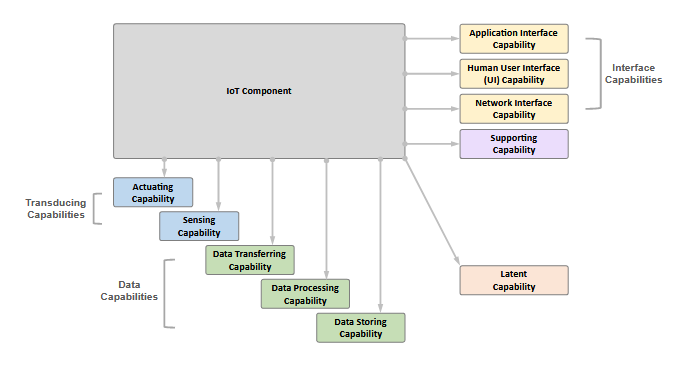
\includegraphics[width=\linewidth]{pic/IIRA-model-component-pattern.png}
	\caption{Component Capability Pattern. \\ (Young et al., 2022, S. 40)}
	\label{fig:Model-Component-Pattern}
\end{figure}
\subparagraph{Three-Tier Architecture Pattern}
The system comprises the Edge, Platform, and Enterprise Tiers, as well as connecting networks. The Edge Tier contains sensors and gateways that collect data. These are connected by the Proximity Network. Data preprocessing may already be happening there.
\\The Platform Tier is responsible for most data processing and storage via databases. It is connected to the Edge Tier via the Access Network.
\\The Enterprise Tier provides domain-specific applications and interfaces for end users. These are built upon the processed data from the platform tier. It also issues controls to lower tiers. This tier is connected to the Access Network via the Service Network.
The three tiers can also be further divided into different domains. That makes sense for bigger systems. But for a simple system as the one described in this work it is not necessary and therefore these domains will not be explained here.
\begin{figure}[H]
	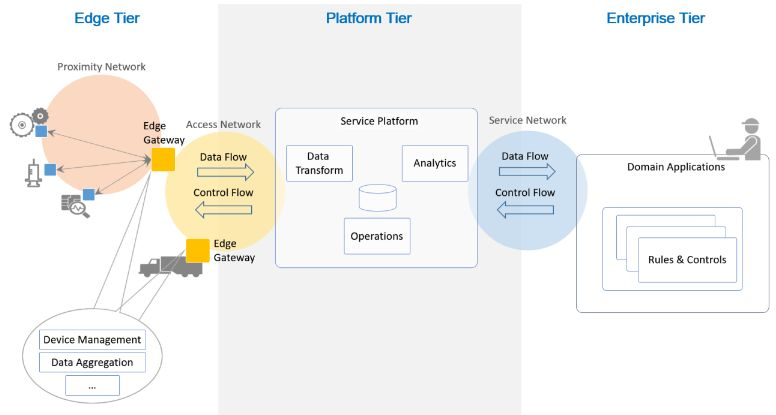
\includegraphics[width=\linewidth]{pic/three-tier-architecture.jpg}
	\caption{Three Tier Architecture \\ (Young et al., 2022, S. 44)}
	\label{fig:Three-Tier-Architecture}
\end{figure}
\subsection{KPIs and Metrics for Performance Evaluation in Sewing Operations}
Performance measurement in the textile production industry is important due to intense competition. It enables producers to identify potential bottlenecks, provides a deeper understanding of processes, and facilitates more effective resource allocation \cite{alauddinProcessImprovementSewing2018}.
\\Key performance indicators (KPIs) and metrics serve as essential tools for performance measurement. Kang et al. \cite{kangHierarchicalStructureKey2016} from the National Institute of Standards and Technology in the United States analyzed the relationships among various types of KPIs and metrics used in operations management and production, based on the ISO 22400 standard.
Supporting elements, referred to as metrics in this thesis, describe the measured data necessary for calculating basic KPIs. These supporting elements are categorized into time and quantity.
Time elements quantify the duration of various events, such as the production time per unit. Conversely, quantity elements pertain to the number of produced items.
Maintenance elements capture information about machine-related issues. 
\\Based on the supporting elements, basic KPIs can be calculated. These KPIs are categorized into production, quality, and maintenance KPIs.
\\The researchers also emphasize the importance of comprehensive KPIs, which provide a broader overview of production performance. These KPIs build upon basic KPIs and include, for example, Overall Equipment Effectiveness (OEE), which is calculated by multiplying the KPIs for availability, performance, and quality ratio.
\\Other studies \cite{kironKPIKeyPerformance2022, alauddinProcessImprovementSewing2018} have specified KPIs specifically for the sewing section of a textile production plant. In this context, some KPIs overlap with those examined by Kang et al., while additional KPIs unique to the sewing section have also been introduced. The following table classifies these sewing-specific KPIs within the hierarchical framework proposed by Kang et al.
\begin{longtable}{|p{3cm}|p{7cm}|p{4cm}|}
	\caption{Classification of KPIs and Metrics in Sewing Section (based on Kang et al., 2016 and ISO 22400)} \\
	\hline
	\textbf{KPI/Metric} & \textbf{Description} & \textbf{Classification (Kang et al., 2016 / ISO 22400)} \\
	\hline
	\endfirsthead
	
	\hline
	\textbf{KPI/Metric} & \textbf{Description} & \textbf{Classification (Kang et al., 2016 / ISO 22400)} \\
	\hline
	\endhead
	% --- Supporting Element: Time ---
	\multicolumn{3}{|l|}{\textbf{Supporting Element: Time}} \\
	\hline
	Cycle Time & Total time taken to complete one operation, from start to start of the next piece. & Supporting Element: Time \\
	\hline
	Standard Minute Value (SMV) & Time required to complete a specific job under standard conditions and pace. & Supporting Element: Time \\
	\hline
	Allowance & Extra time permitted for personal needs, delays, and fatigue in production. & Supporting Element: Time \\
	\hline
	Idle Time/Machine & Time when operators or machines are not working, considered lost time. & Supporting Element: Time \\
	\hline
	% --- Supporting Element: Quantity ---
	\multicolumn{3}{|l|}{\textbf{Supporting Element: Quantity}} \\
	\hline
	Operation & A step in the process required to convert materials into a finished product. & Supporting Element: Quantity \\
	\hline
	Manpower to Machine Ratio & Ratio of workers to machines, used to optimize labor and production. & Supporting Element: Quantity \\
	\hline
	Absenteeism & Rate of operator absence, which affects production and efficiency. & Supporting Element: Quantity \\
	\hline
	No of Style Change & Frequency of style changes, impacting productivity, efficiency, and quality. & Supporting Element: Quantity \\
	\hline
	% --- Basic KPI: Production ---
	\multicolumn{3}{|l|}{\textbf{Basic KPI: Production}} \\
	\hline
	Efficiency & Comparison of actual output to what could be achieved with the same resources. & Basic KPI: Production \\
	\hline
	Productivity & Achievement toward goals based on the relationship between inputs and outputs. & Basic KPI: Production \\
	\hline
	Availability & Percentage of scheduled time employees or machines are productive. & Basic KPI: Production \\
	\hline
	Performance & Amount of product delivered relative to available productive time. & Basic KPI: Production \\
	\hline
	Line Wise Sewing Efficiency & Efficiency of sewing lines, often linked to man-to-machine ratio. & Basic KPI: Production \\
	\hline
	% --- Basic KPI: Quality ---
	\multicolumn{3}{|l|}{\textbf{Basic KPI: Quality}} \\
	\hline
	Defect per Hundred Units (DHU) & Number of defects found per hundred units produced. & Basic KPI: Quality \\
	\hline
	Quality & Percentage of perfect or saleable products produced. & Basic KPI: Quality \\
	\hline
	% --- Comprehensive KPI ---
	\multicolumn{3}{|l|}{\textbf{Comprehensive KPI}} \\
	\hline
	Overall Labor Effectiveness (OLE) & Measures workforce utilization, performance, and quality, reflecting labor's impact on productivity. & Comprehensive KPI \\
	\hline
	Overall Equipment Effectiveness (OEE) & Quantifies how well equipment performs relative to its designed capacity, considering availability, performance, and quality. & Comprehensive KPI \\
	\hline
\end{longtable}
\subsection{IoT-Plattforms}
The IoT is known for producing large amounts of data and for the potentials to grow these amounts even more. Therefore a scalable software infrastructure that is needed. That is where IoT-Plattforms come into play \cite{turkiEvaluatingOpenSource2024}. The authors also mention that IoT-Platforms help accelerating the solution development "[...] by providing foundational capabilities, avoiding the need to implement low-level infrastructure."
\\\cite{asemaniUnderstandingIoTPlatforms2019} further highlight the different capabilities that are typical for IoT-Platforms.
\paragraph{Connectivity and Device Management}
Through various communication protocols the platforms connect with the devices, enabling them to communicate with each other, manage device status and configurations, handle software updates and provide mechanisms for error reporting.
\paragraph{Data Storage, Management, Analysis, Visualization}
Through connections to databases they store large volumes of data often in the cloud or locally. Also further data processing and analytics through various methods as well as visualizations through dashboards are possible.
\paragraph{Development and Deployment Tools}
By providing APIs and SDKs the developers are enabled to further create custom applications.
\paragraph{Auditing and Payments}
The Platforms help to have an overview over the data or compute usage and the resulting costs.
\paragraph{Service Management}
By giving an oversight over parameters like resource consumption, data requirements and access, the user can monitor vertical as well as platform internal services. The platforms also enable the communication between services or combination of basic services to create new ones.
\paragraph{Integration}
Platforms can be integrated with each other, other data sources and the cloud. 
\paragraph{Fog/Edge Computing}
IoT-Platforms often support distributed data processing and storage. This can lead to less traffic due to processing close to the data source. Faster transmission would be enabled therefore and reinforced due to  shorter communication distances.
\\\\The researchers go on to reveal that while commercial platforms carry all of the mentioned capabilities, open source platforms are often focused on specific capabilities. Thus in implementation sometimes need to be combined to deliver a holistic IoT-Platform. 
\subsection{Differences between Relational and Timeseries Databases}
In the paper written by \cite{turkogluComparisonTimeSeries2024} it is analyzed how relational databases and time series databases compare regarding speed and storage efficiency when used in Grafana.
First they point out the use case for relational databases is for single time data points, which can be related to other data points over various tables. Therefore enabling complex queries involving joins, aggregations and multiple tables. They make sure the data is accurate and stays consistent.
Time series data bases on the other hand are made for data points with a timestamp and large volumes of data. This makes them ideal for IoT applications and real time data analytics. They are optimized to enable high speed read and write operations as well as efficient data storage.
The differences in query return time are already there with small amounts of data, but when scaling up the amount they become clearly visible as can be seen in the figure below.
\begin{figure}[H]
	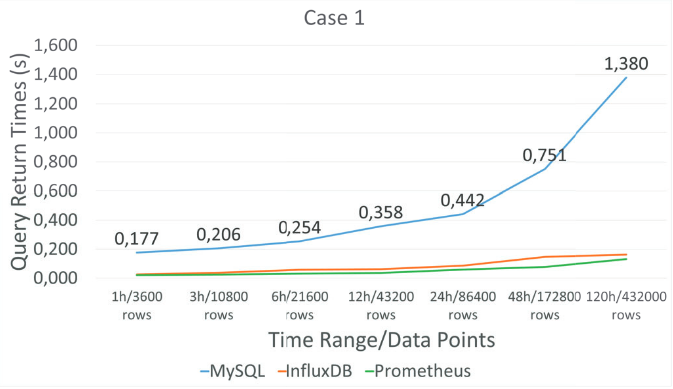
\includegraphics[width=\linewidth]{pic/query-performance-db.png}
	\caption{Query Performance Relational vs. Time Series DB \\ (Turkoglu et. al, 2024, S. 2)}
	\label{fig:query-performance-db}
\end{figure}
This is only one of three test cases but they all give a similar picture that shows the superiority of time series databases regarding query return times.

\subsection{Dashboarding}
\addtocontents{toc}{\vspace{0.8cm}}



\clearpage
\chapter{\textbf{Related Work}}\label{relatedWork}
This section presents an overview of related solutions for sewing machines, with a focus on methods for data collection and processing in monitoring applications. It also examines general approaches to performance measurement in manufacturing. The analysis will likely address the types of metrics underlying these solutions, the sensor technologies used for data acquisition, and the strategies for data processing, storage, and analytics. This review aims to clarify the current state of the art, identify possible gaps in existing systems, and position this work within the field of automated performance measurement systems. Furthermore, the review seeks to highlight potential limitations and opportunities, including technical aspects such as hardware, software, and integration, as well as architectural considerations like standards, frameworks, and open-source approaches, which may influence the implementation of performance measurement systems.
\\\\
In their seminal work, Jung et al. \cite{jungRemoteSensingSewing2020} propose a system for the analysis of sewing machine operator skill level and the complexity of the assigned sewing tasks. The present study bears a notable similarity to the aforementioned work, as both analyze the cycle time per unit. This objective is pursued by employing power consumption data of the sewing machines as the fundamental metric. To that end, a power monitoring system is employed, which is connected to the machines power plug without necessitating modifications to the sewing machine itself. Subsequently, the data is transmitted to a cloud server via wireless communication. The determination of quantity and time of work is achieved through the implementation of pattern analysis algorithms. The efficacy of the system is predicated on the non-intrusive nature of PMS. A notable disadvantage of this solution is the necessity of sufficient sample data to ensure the accuracy of the results.\\
Another system that uses power consumption measurement was proposed by Strazinskas \cite{strazinskasDevelopmentSolutionMonitoring2025}. The utilization of current sensors enabled the discernment of fluctuations in motor current, which are inherently associated with the operational states of the sewing machine, including initiation, cessation, seam length, and stitch speed. The sensor is connected to an Arduino Uno microcontroller, which transmits the received data to a Raspberry Pi 3B+ microcomputer. The microcomputer is responsible for central data collection and storage. The data is stored in files, which is a disadvantage of the system because it is less efficient than storing it in an optimized time series database. Therefore, a greater quantity of space is required, and the rate of data processing is reduced. Additionally, the absence of any preprocessing mechanisms underscores the necessity for optimized data management, a crucial aspect that demands significant memory resources. Strazinskas's research indicates that the utilization of the present sensor engenders measurement errors and noise in the data.\\
Although adopting a divergent approach, the system proposed by Quoc et al. \cite{quocApplyingIoTOperations2025} likewise relies on IoT devices (which were not further described) connected to the machine. The data of these devices is then transmitted to the cloud, where it is integrated with the enterprise's Management Information System (MIS). This integration facilitates the optimization of resource allocation. In light of the aforementioned data, a visualization is generated to illustrate the open positions of a contract and the extent to which it has been completed.\\
A divergent approach is posited by Wedanage et al. \cite{wedanageFogAssistedIndustrial2022} in their study "Fog Assisted Industrial Sewing," in which they utilize a mobile application to record the cycle times of the sewing step.To initiate and conclude the sewing process on the workpiece, the operator is required to engage a designated button at the commencement and cessation of the operation. The data is structured in a JSON format and published via MQTT under a designated topic. A fog node, implemented using a Cisco IR829 industrial router, is subscribed to the specified topic and processes the data through a Java application. Additionally, the application utilizes a RethinkDB database, which is characterized as open-source and specifically engineered for real-time applications. The fog node is already capable of performing local data analytics. In the cloud, data from all fog nodes is combined to provide real-time alerts and analytics through dashboards. These dashboards visualize cumulative average cycle times per member and compare them to takt time (maximum time allowed to produce one product to meet customer demand). The employment of fog computing facilitates the system's notable scalability, a consequence of the distribution of computing tasks across multiple fog nodes. This configuration facilitates the system's capacity for real-time data analytics and reduced bandwidth utilization. A notable drawback of this system is its reliance on manual input from operators, which introduces a margin of error. Moreover, no historical analytics have been conducted, despite the existence of a foundation for such analyses.
A notable drawback of the system in question, as well as those proposed by Jung et al. and Quoc et al., is the utilization of a cloud, which gives rise to several concerns, including but not limited to data security, latency, and ongoing costs.
The merits of the aforementioned systems include their capacity for retrofitting older machines and their non-intrusive nature.
\\\\
Beyond these closely related implementations, a broader perspective is provided by Tambare et al. \cite{tambarePerformanceMeasurementSystem2022}, who review various approaches to performance measurement systems. Initially, the discourse centers on two pivotal standards. The ISA-95 standard delineates entities at the shop floor level, where information technology systems such as ERP, CRM, cloud platforms, and SQL databases interact with operational technology components like sensors, actuators, microcontrollers, SCADA systems, and PLCs. Its primary function is to formalize production processes. Conversely, the ISO 22400 is employed for the formalization of performance metrics. The provided framework facilitates the definition, calculation, and dissemination of key performance indicators (KPIs), encompassing their contextual framework, formula, unit of measurement, range, and intended audience. The researchers then proceed to underscore the Scania case study, wherein these two standards are being utilized, as a paradigm of the practical implementation of international standards for performance measurement in a smart manufacturing context.\\
This case study by Samir et al. (samirKeyPerformanceIndicators2018) will now be examined in more detail. The system is composed of numerous autonomous, self-contained computational units that are each capable of performing independent computations and collaborating with each other. The software utilized for the processing and distribution of data has been developed using a Service Oriented Architecture (SOA) framework. This approach involves the implementation of multiple services that function independently of one another, with each service designated to specific responsibilities. The communication between the units is facilitated by an Enterprise Service Bus (ESB). The architecture further employs an Event-Driven Architecture (EDA), whereby events serve as triggers for services. This aims to address the issue of communication delays. The KPIs are designed in accordance with the ISO 22400 standard, and the IS-95 is employed to enable automated interfaces between enterprise and control systems.
\\\\
Taken together, these studies illustrate a variety of approaches to IoT-based machine monitoring, each with specific strengths and limitations.
In contrast to the systems examined in the aforementioned studies, the system presented in this thesis is designed to operate with a contemporary sewing machine that facilitates data extraction directly from the machine. It is also intended to provide a more comprehensive overview of the production process by means of various Key Performance Indicators (KPIs), which will be addressed in subsequent sections.
The system proposed in this thesis aims to incorporate the strengths of the discussed systems while mitigating their weaknesses. The system has been designed to align more closely with the proposed model in the case study by implementing standards and service-oriented software. Therefore, this facilitates enhanced scalability and maintainability.


\chapter{\textbf{Requirements Analysis}}\label{grundlagen}
In order to select the most suitable technologies and design the system, it is first necessary to establish clear requirements. In this chapter, the aforementioned requirements will be enumerated and elucidated.
In order to maintain consistency regarding the compliance level, the terms "must," "should," and "will" were employed.
The following words shall be explained in brief. The term "must" is employed to signify an unconditional obligation, implying that the fulfillment of this requirement is not subject to discussion or negotiation. The term "should" conveys a degree of desirability, indicating that fulfillment of the requirement would be advantageous. The term "will" signifies that this particular requirement is currently under consideration for inclusion in the subsequent release. However, it is imperative to maintain awareness of this requirement so that the system can be designed in a manner that facilitates its seamless integration in the future.
\subsection{Functional System Requirements} % (from your requirements table)
\begin{tabularx}{\textwidth}{|X|X|}
	\hline
\textbf{Requirement}	& \textbf{Explanation} \\
	\hline
The system must show KPIs that are relevant for the sewing process	&  In the workshops there must be some KPIs that fit into the story of a textile production with a sewing process\\
	\hline
The system should show aditional KPIs that are relevant for the manufacturing industry in general	&  Workshop participants are from all sorts of companies within the manufacturing industry\\
	\hline
 The system must present these KPIs in a visual manner that provides information about the classification of the current value e.g. with colors and thresholds	& So that the management can act quickly upon the KPIs and does not need to lookup thresholds \\
	\hline
The system must provide the user with the ability to change the timeframe on which the KPIs are calculated	&  Especially when looking at historic data it is usefull to be able to set the timeframe\\
	\hline
The system should show graphs with historical data & Enables management to see trends and patterns\\
	\hline
\end{tabularx}

\subsection{Non-Functional Requirements} %(scalability, security, real-time processing)
\begin{tabularx}{\textwidth}{|X|X|}
	\hline
\textbf{Requirement}	&  \textbf{Explanation}\\
	\hline
The system must make use of open source software where possible	&  To be replecable by small and medium companies\\
	\hline
The system must be capable to generate all of the KPIs from the machine-data without installing any additional sensors	&  \\
	\hline
The system must be designed in a way that makes it easily scalable	&  \\
	\hline
The system must be deployable with minimal effort	&  \\
	\hline
The system must be capable to retrieve raw data via opc-ua	&  \\
	\hline
The system should make use of existing patterns, frameworks and solutions were possible	&  \\
	\hline
The system should update the KPIs in real-time (<10s)	&  \\
	\hline
 The system must be able to run on a local machine and therefore independent of any cloud service	&  \\
	\hline
The system must provide the user with the ability to access the dashboard from within the shopfloor network	&  \\
	\hline
\end{tabularx}

\subsection{Constraints} %(no additional sensors, existing infrastructure)
\subsection{KPI Selection and Justification}
 Of which the following were able to be calculated with the given metrics.
\\
\clearpage
\chapter{\textbf{Implementation}}\label{Implementation}
\section{Sewing Machine Signal Connection and Data Acquisition}
The final signals necessary to calculate all selected KPIs are "Thread Trimming," "Pressure foot," "Upper shaft rotating," and "Main menu and not sewing." The retrieval of these signals was contingent upon their initial assignment to the correct output pins in the machine's menu configuration. The subsequent challenge was to establish a connection between the output pins and the input pins of the WAGO PLC.

A connection for one signal from the sewing machine had already been established during an earlier project, but unfortunately, the connection was inadequately documented. This proved to be more confusing than helpful. The connection was implemented as follows: The signal pin of the sewing machine was connected to the 0V reference of the PLC. The 24V pin of the sewing machine was connected to the signal input connector of the PLC. Figure 5.1 provides a visual aid to facilitate comprehension of this configuration. This arrangement made sense once it was discovered that the sewing machine signals are NPN type, while the PLC exclusively accepts PNP signals as input. Typically, when the sewing machine would also have signals of type PNP, the signal pins would simply be connected to the signal connectors of the PLC. Concurrently, the 0V connector of the PLC would be connected to the GND pin of the sewing machine.
\begin{figure}[H]
	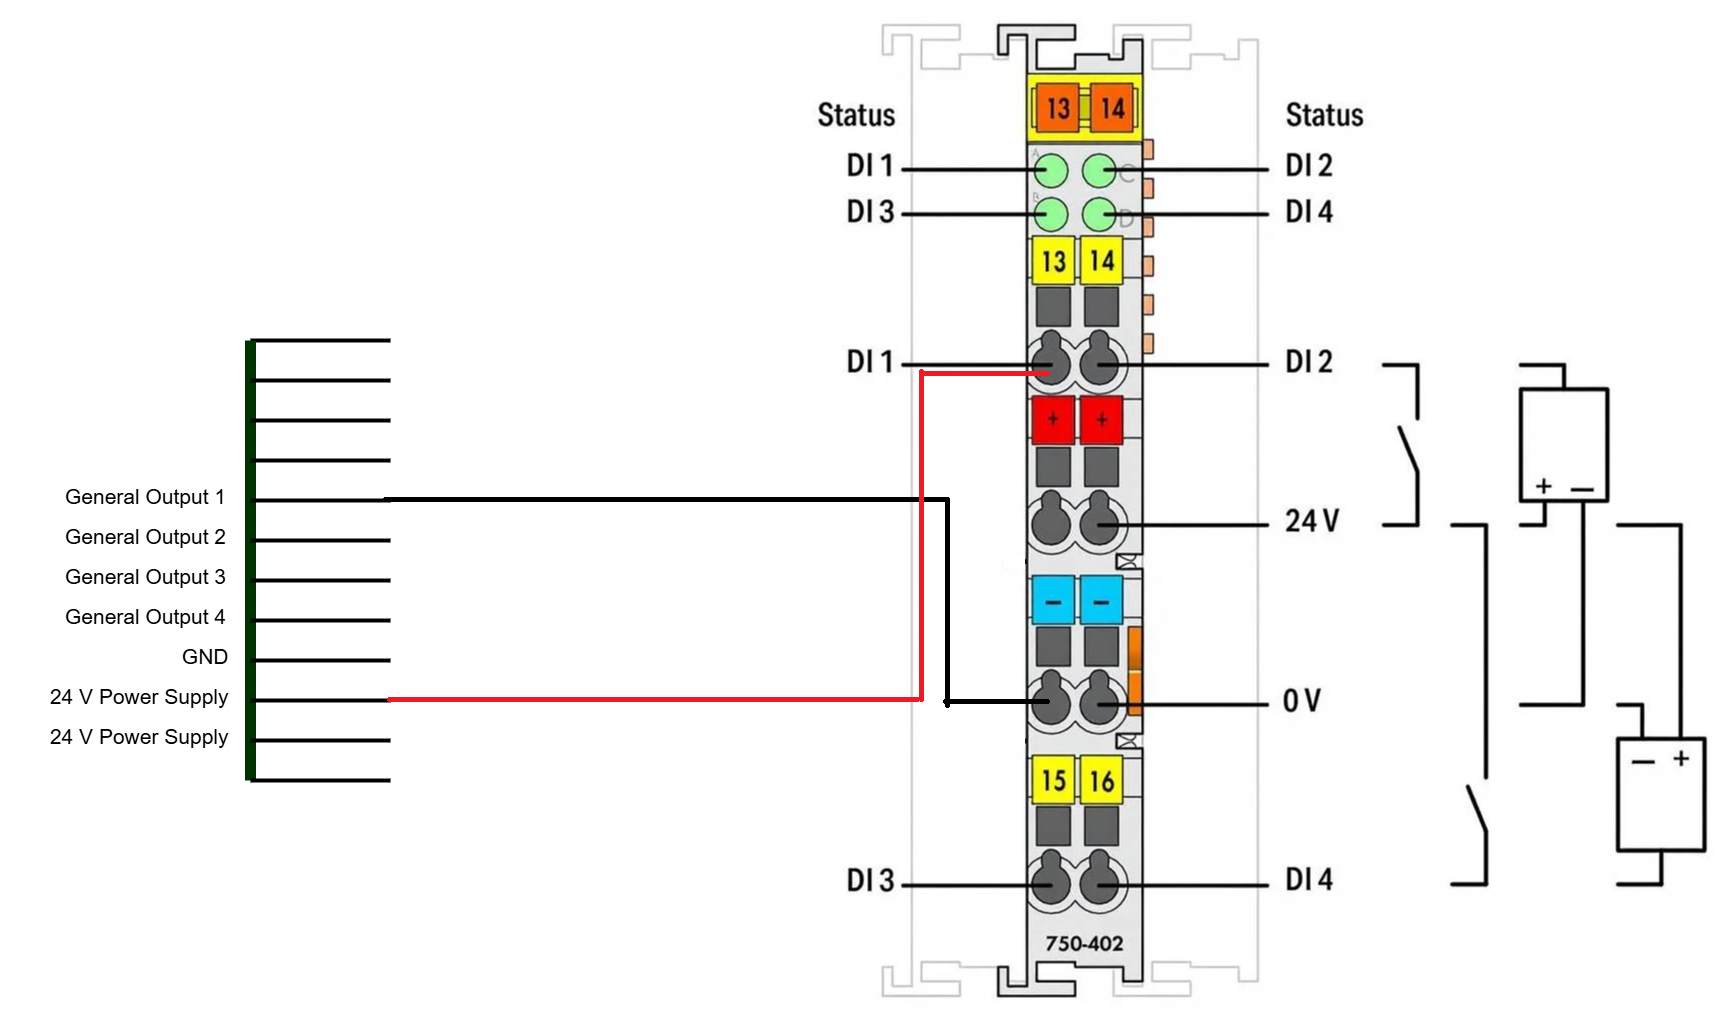
\includegraphics[height=7.4cm]{pic/sewing-machine-plc-init.png}
	\caption{Initial Connection of Sewing Machine to PLC}
	\label{fig:Model-Component-Pattern}
	\small\textit{Note: The 12-pin connector of the sewing machine is located on the left side. This connector contains various pins, including those that function as signal pins. The left side of the module contains the PLC input module. The DI1-4 marked connectors of the PLC serve the function of signal input connectors.}
\end{figure}
The system was configured so that when a signal becomes active, it draws current through the signal input connector of the PLC, resulting in a high signal. However, this implementation was limited to only two signals, because there is only one 0V connector available for two signal input connectors. In total, there are two 0V connectors and four signal input connectors. When two 24V pins are connected to one 0V connector via the signal input pins, an active signal draws current through the 0V connection and simultaneously pulls current from both input signal connectors. This results in invalid signals. 


The resolution of the aforementioned issue necessitated the conversion of the NPN signals of the sewing machine into PNP signals, which are compatible with the PLC. For the execution of this task, an optocoupler was utilized. The implementation was executed in accordance with the subsequent description. Subsequently, the signal output pins of the sewing machine were connected to the signal input connectors of the optocoupler. Furthermore, a connection to the 24-V power supply of the sewing machine was established for each signal input. The signal connectors on the output side of the optocoupler are connected to the signal input connectors of the PLC. Concurrently, the 24-V power supply of the PLC is connected to the VCC input connector of the optocoupler. Additionally, the 0V connector of the programmable logic controller PLC is linked to the GND connector of the optocoupler. The wiring of the optocoupler can be observed in the following Figure.
\begin{figure}[H]
	\centering
	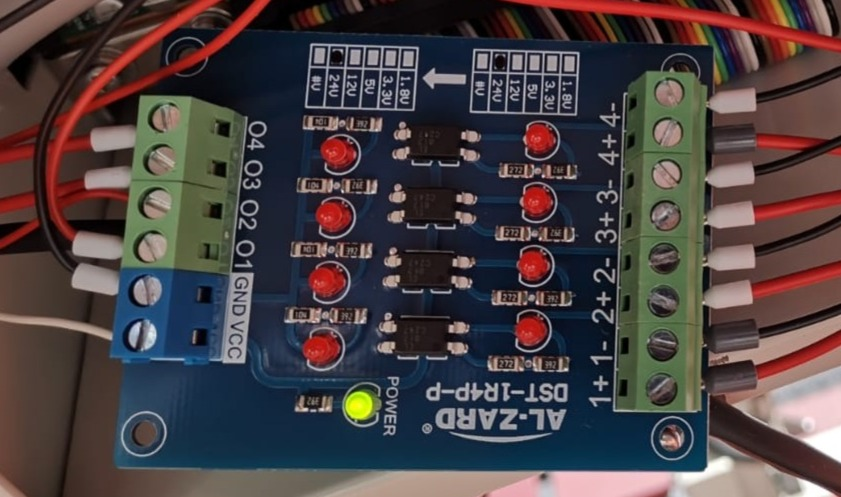
\includegraphics[height=6cm]{pic/optocoupler-wiring.jpg}
	\caption{Initial Connection of Sewing Machine to PLC}
	\label{fig:Model-Component-Pattern}
\end{figure}
As illustrated, the red cables represent electrical connections originating from or terminating at a 24V power source. Additionally, the white cable located on the left side is linked to the 24V source of the PLC. The black cables serve as connections to ground or to the signal pins on the right side. These connections function in a manner that pulls down the current when signals are in a state of activity.
In order to ensure the signal's availability across the shopfloor network, it was imperative to program the PLC in a manner that facilitated this objective. The input signals simply needed to be assigned to a value and then published over OPC UA. \\
Initially, only the IP address and the OPC UA port of the PLC were known. In order to enhance comprehension regarding the retrieval of data from the aforementioned system through the utilization of an OPC UA client, the development of a Python script was undertaken. The script under consideration took the two givens, established a connection, and navigated through the OPC UA server's node structure. The search is conducted for a "DeviceSet" node, which is understood to generally contain industrial devices, such as sewing machines. For each device identified, an exploration of its variables and child objects is initiated. It is important to acknowledge that, at this juncture, the connection from the preceding project was still in place. Further exploration was necessary to ascertain the nature of the connection and to identify any additional machines that were connected to the PLC. At this time there was a delay in communication with "Brother Internationale Industriemaschinen GmbH." Therefore, the necessary information regarding the configuration of the sewing machine signals was not available. A decision was reached to initiate an exploration of effective communication methods with the OPC UA server.\\
Subsequent to the establishment of a connection to the PLC for all signals, a diagnostic procedure was conducted to ascertain the availability of all signals. For this purpose, a tool known as UAExpert was utilized. The software under discussion is an OPC UA client that provides a user interface for development, testing, and monitoring. The device was utilized for the purpose of monitoring the values of the signals. Consequently, the actions that were expected to elicit the signals were executed on the sewing machine. Initially, the process was proceeding according to plan. -	However, after a certain period, one of the signals ceased functioning, resulting in a persistent display of the value "false". Therefore, it was necessary to measure the current in order to ascertain the location of the failure. It was observed that a short circuit occurred on the printed circuit board (PCB) during the measurement process. The probable rationale pertains to an inadvertent connection between two 24-volt sources through the utilization of a multimeter.  Subsequent to the incident, retrieval of the signals from the sewing machine was rendered unfeasible. A decision was made to simulate the OPC UA server and generate test data that would emulate the standard sewing process. The decision was made to implement the system in a manner that would allow for the subsequent connection of the sewing machine to the data processing and analytics system following the installation of a new PCB.

\section{Data Preprocessing}
\begin{figure}[H]
	\centering
	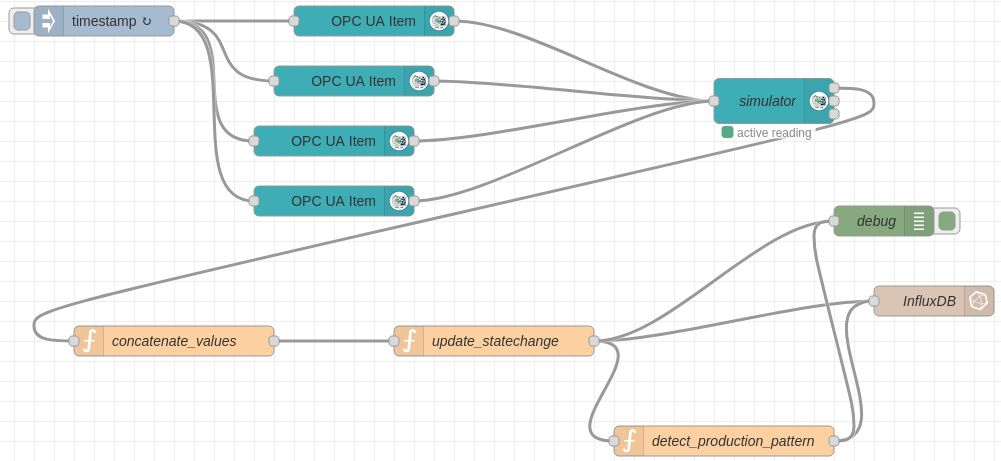
\includegraphics[height=7cm]{pic/node-RED.jpg}
	\caption{Data retrieval and preprocessing}
	\label{fig:Model-Component-Pattern}
\end{figure}
In the context of this study, Node-RED was utilized as a service to retrieve data that had been published by the PLC's OPC UA server. This feature facilitates the preprocessing and subsequent injection of data into the database. The retrieval of data from the OPC UA server is facilitated by an OPC UA package known as "node-red-contrib-opcua." The node designated as "timestamp" at the inception of the flow serves merely to initiate the flow. The temporal configuration of this feature may be set to various intervals or fixed times. The decision was made to establish an interval of 0.2 seconds. This interval was selected due to the fact that some operations on the sewing machine have an execution time of approximately one second when operated by inexperienced workers. In light of the dearth of seasoned professionals, it was deduced that an experienced worker would exhibit a fourfold increase in efficiency. To ensure the capture of all events, the interval was set to 0.2 seconds, equivalent to the execution time of a worker operating at a rate five times faster. Subsequent to the completion of the trial, the interval may be recalibrated in accordance with the findings of the evaluation. The four subsequent nodes, designated as OPC UA Items, each contain the namespace and ID of the various signals. These are subsequently fed into the simulator node. The node in question has been configured with the endpoint, which consists of the IP address of the PLC, the port, and the name of the OPC UA server, if such a server exists. This node is responsible for generating the values for each of the OPC UA items in a serial manner.
The succeeding node is one of three function nodes. These function nodes contain JavaScript code that executes three distinct preprocessing steps. The initial step involves the concatenation of the four values into a single string. The primary rationale for concatenating values is that, in InfluxDB, each value is assigned its own table. In the event that a query is executed over a set of values, the tables must be joined, a process that is computationally intensive. This phenomenon can result in substantial delays in the final dashboard. The concatenation of values eliminates the necessity for joining tables, as all values are subsequently stored within a single table.
This preprocessing step confers an additional advantage, namely that it facilitates the subsequent step in the procedure. The subsequent preprocessing step in the function node designated "update\_statechange" involves the verification of whether the concatenated string undergoes alterations. A modification in the configuration of the string is indicative of a state alteration in the sewing machine. Consequently, the string undergoes an output transformation. The initial concatenation of the values reduces the number of comparisons from four to one string. This preprocessing step was implemented to reduce the amount of data stored in the database. In previous iterations, this step was omitted, resulting in a substantial reduction in query processing speed relative to subsequent iterations. The output of the second preprocessing node is comprised of four separate key-value pairs of the signals, as well as these in a concatenated string format. It is important to note that these values are only provided as output when there is a change in one of the values compared to the previous state. The output of this node is utilized as an input for the third preprocessing node.
In the preceding section (4.0.7), the production pattern was delineated as a metric for quantifying the duration of machine utilization for value-adding operations. The final preprocessing node, designated "detect\_production\_pattern", serves to ascertain the presence of this pattern. The output of this function is the key "pattern" with a value of true, indicating the beginning of the pattern, or false, indicating the end of the pattern. Additionally, the timestamp indicating the end or beginning of the pattern is included in the output.
Upon completion of the data flow, both outputs from the "updateStateChange" function and the "detect\_production\_pattern" process are transferred to the designated InfluxDB node as input. This node has been configured with the address and the API key of the Influx database. The component in question is an InfluxDB out node, which signifies that it is capable of writing data exclusively to InfluxDB. This node stems from the node-red-contrib-influxdb package. In the course of each write operation, the system automatically incorporates a timestamp into the input. However, it is imperative to incorporate a timestamp at the "detect\_production\_pattern" node, as the pattern's detection is only possible in a retrospective manner. Consequently, the timestamp of the InfluxDB node would be inadequate.

\section{Data Storage and Post-Processing}
In the context of InfluxDB, it is necessary to establish a designated bucket for the designated project. In the context of a relational database management system (RDBMS), a bucket can be regarded as analogous to a schema. The bucket is configured with a retention policy and access rights. The retention policy is a mechanism that governs the duration for which data is retained in the bucket. The preliminary step in the process was the creation of an initial bucket, into which data was subsequently streamed from Node-RED. Initially, an unlimited retention policy was configured for the specified bucket. Subsequently, in light of apprehensions pertaining to an excess of data, the determination was made to curtail the retention policy to a span of one day. Following the initialization of the process, the data of the first bucket is aggregated and stored in a separate bucket that employs an unlimited retention policy. The aggregation process leads to a substantial reduction in the amount of data that must be stored. Aggregation is performed within designated tasks. These tasks can be configured to execute either upon the completion of a specified time interval or through the utilization of cron syntax, which facilitates the establishment of a predetermined time for regular aggregation. The latter is employed in this implementation. The rationale underlying this necessity is that it is imperative for the aggregation to occur during the period between the conclusion of one shift and the commencement of the subsequent one. This phenomenon can be attributed to the prevalence of data aggregation processes that are contingent upon the identification of the initial and concluding points of an event. In the case that the aggregation occurred between these events, the result would be a falsification. The aggregation could also be executed at eight-hour intervals, thereby aligning with the duration of a typical shift. However, given the legal framework delineated in the foundational chapter, the daily aggregation is applied. The implementation of an eight-hour aggregation period would result in the accumulation of data that could be traced back to a specific worker. The aggregation of data over the course of an entire day encompasses three shifts. Consequently, it is not possible to draw any conclusions from the data regarding the individual performance of a worker. A notable benefit of this approach is a significant reduction in the necessary storage capacity, amounting to approximately two-thirds of the original requirement.
The aggregation of these data is facilitated by the utilization of the flux query language. Throughout the developmental process, the aggregations were meticulously formulated in flux notebooks. These notebooks bear a resemblance to Jupyter notebooks and can be utilized within the web user interface of the InfluxDB DBMS. Cells for flux queries and additional cells for visualizing the result or displaying the resulting table(s) can be added to the notebook. In this manner, the proper functioning of the query can be readily corroborated. A thorough exposition of the methodology employed for the verification of results can be found in the Evaluation chapter. The results of the aggregations encompass all of the supporting elements.

\subsection{Flux Query Language}
\begin{lstlisting}[style=FluxStyle, caption={Flux aggregation query for produced quantity}]
from(bucket: "sewing-machine-1-simulated")
|> range(start: -24h)
|> filter(fn: (r) => r["_measurement"] == "sewingMachine1")
|> filter(fn: (r) => r["_field"] == "thread_trimming" and r["_value"] == true)
|> count()
|> map(fn: (r) => ({r with _time: now()}))
|> map(fn: (r) => ({r with _field: "pieces"}))
|> to(bucket: "simulated-tasks")
\end{lstlisting}
A comparison of the flux query language with SQL-like query languages reveals notable distinctions in their respective syntax and semantics. Accordingly, the fundamental principles of flux querying are elucidated herein. The initial step in the process is the selection of the bucket from which the data is to be utilized for processing, as illustrated in the initial row. The "|>" (pipe forward) symbol is employed in each subsequent row. This operator indicates that the result of the preceding operation is to be utilized in the subsequent operation. The subsequent row is designated for the specification of the timeframe for the desired data. This is a common practice at the outset to minimize data and, consequently, processing time. Furthermore, the subsequent filtration operations function in a similar manner, thereby allowing for the selection of only the pertinent data. The "\_measurement" constitutes a logical grouping of the data, encompassing numerous tags and fields. The utilization of tags facilitates the creation of additional data groups. For instance, in the event that a project encompasses multiple sewing machines, the measurement name could be altered to "State," and the tag could contain the names of the identifiers for each sewing machine.  Fields are defined by a name and a value, and their distinguishing characteristic is that they undergo changes over time. Subsequent processing of the data typically occurs subsequent to the filtration stage. The number of operations that can be chained together is unlimited. The count operation in this particular instance is one of numerous aggregate functions that reduce the quantity of values to a single value. The map function can be used to apply a function to every row in a data set. Upon completion of the query, the final result is returned. In this particular instance, the result is written to an alternate bucket.







\clearpage
\chapter{\textbf{Zusammenfassung und Ausblick}}\label{zusammenfassung}
\addtocontents{toc}{\vspace{0.8cm}}


% Nachspann
\nocite{Segmentation} % Quelle wird nicht im Text erwähnt -> Quellenverzeichnis
\nocite{ImageAttack}
% Weitere quellen müssen in 'bib/quellen.bib' eingetragen werden
% !!! -> BibTex ausführen! Sonst tauchen die Quellen nicht im Verzeichnis auf.

% Quellenverzeichnis
\clearpage
%\bibliographystyle{alpha}
\bibliographystyle{apalike}
\bibliography{./bib/quellen}
\addcontentsline{toc}{chapter}{Quellenverzeichnis}
%\addtocontents{toc}{\vspace{0.8cm}}

% Abkürzungsverzeichnis
\clearpage
\markright{Abkürzungsverzeichnis}
\clearpage
\chapter*{Abkürzungsverzeichnis}\label{abkuerzungsverzeichnis}
\addcontentsline{toc}{chapter}{Abkürzungsverzeichnis}
\begin{acronym}[YTM]
\setlength{\itemsep}{-\parsep}

\acro{IoT}[$IoT$]{\hspace{1cm}Internet of Things}
\acro{IIoT}[$IIoT$]{\hspace{1cm}Industrial Internet of Things}
\acro{KPI}[$KPI$]{\hspace{1cm}Key Performance Indicator}
\acro{PLC}[$PLC$]{\hspace{1cm}Programmable Logic Controller}
\acro{OPC UA}[$OPC UA$]{\hspace{1cm}Open Process Control Unified Architecture}
\acro{DBMS}[$DBMS$]{\hspace{1cm}Database Management System}
\acro{TS-DBMS}[$TS-DBMS$]{\hspace{1cm}Timeseries Database Management System}
\acro{}[$x$]{\hspace{1cm}x}


\end{acronym}

%\addtocontents{toc}{\vspace{0.8cm}}

% Abbildungsverzeichnis
\clearpage
\addcontentsline{toc}{chapter}{Abbildungsverzeichnis}
\listoffigures
%\addtocontents{toc}{\vspace{0.8cm}}

% Tabellenverzeichnis
\clearpage
\addcontentsline{toc}{chapter}{Tabellenverzeichnis}
\listoftables
\addtocontents{toc}{\vspace{0.8cm}}

% Anhaenge
\addcontentsline{toc}{chapter}{Anhang}
\appendix
%\input{./app/Dateiname}
\chapter{Quellcode}
\begin{enumerate}
      \item Source 1
      \item Source 2
\end{enumerate}

% Anhänge im Ordner 'app' ablegen

%\includepdf[pages=1-4]{./app/Datenblatt1.pdf} % Datei mit 4 Seiten
%\includepdf[pages=1]{./app/Datenblatt2.pdf} % Datei mit einer Seite

\chapter{Rohdatenvisualisierungen}
\begin{enumerate}
      \item Graustufen
      \item Verteilungen
\end{enumerate}
\end{document}
